\chapter*{Appendices}
\addcontentsline{toc}{chapter}{Appendices}
\section*{Some Definition in Graph Theory}
\begin{definition}
A \textbf{graph} is a ordered pair of sets $(V,E)$ and $E$ is the set of pair of elements of $V$. A \textbf{directed graph}, or a \textbf{digraph} is a ordered pair of sets $(V,E)$ and $E$ is the set of ordered pair of elements of $V$. And we call $V$ be the set of vertices and $E$ be the set of edges. A \textbf{tournament} is a digraph such that for each pair of vertices we have exactly one edge connecting them.
\end{definition}
\begin{example}
Let $G(V_1,E_1)$ be a graph with vertex set $V_1=\{1,2,3,4\}$ and edge set 
\[E_1=\{(1,2),(2,2),(2,3),(3,1)\}.\]
And let $D(V_2,E_2)$ be a $digraph$ with vertex set $V_2=\{1,2,3,4\}$ and edge set 
\[E_2=\{(1,2),(2,1),(2,2),(2,3),(3,2),(1,3),(3,1),(1,4),(4,3)\}.\]
Finally let $T(V_3,E_3)$ be a digraph with vertex set $V_2=\{1,2,3,4\}$ and edge set 
\[E_3=\{(1,2),(1,3),(1,4),(2,3),(2,4),(3,4)\}.\]
Thus $T$ is a tournament. And we can draw $G$, $D$, $T$ as follow.
\begin{center}
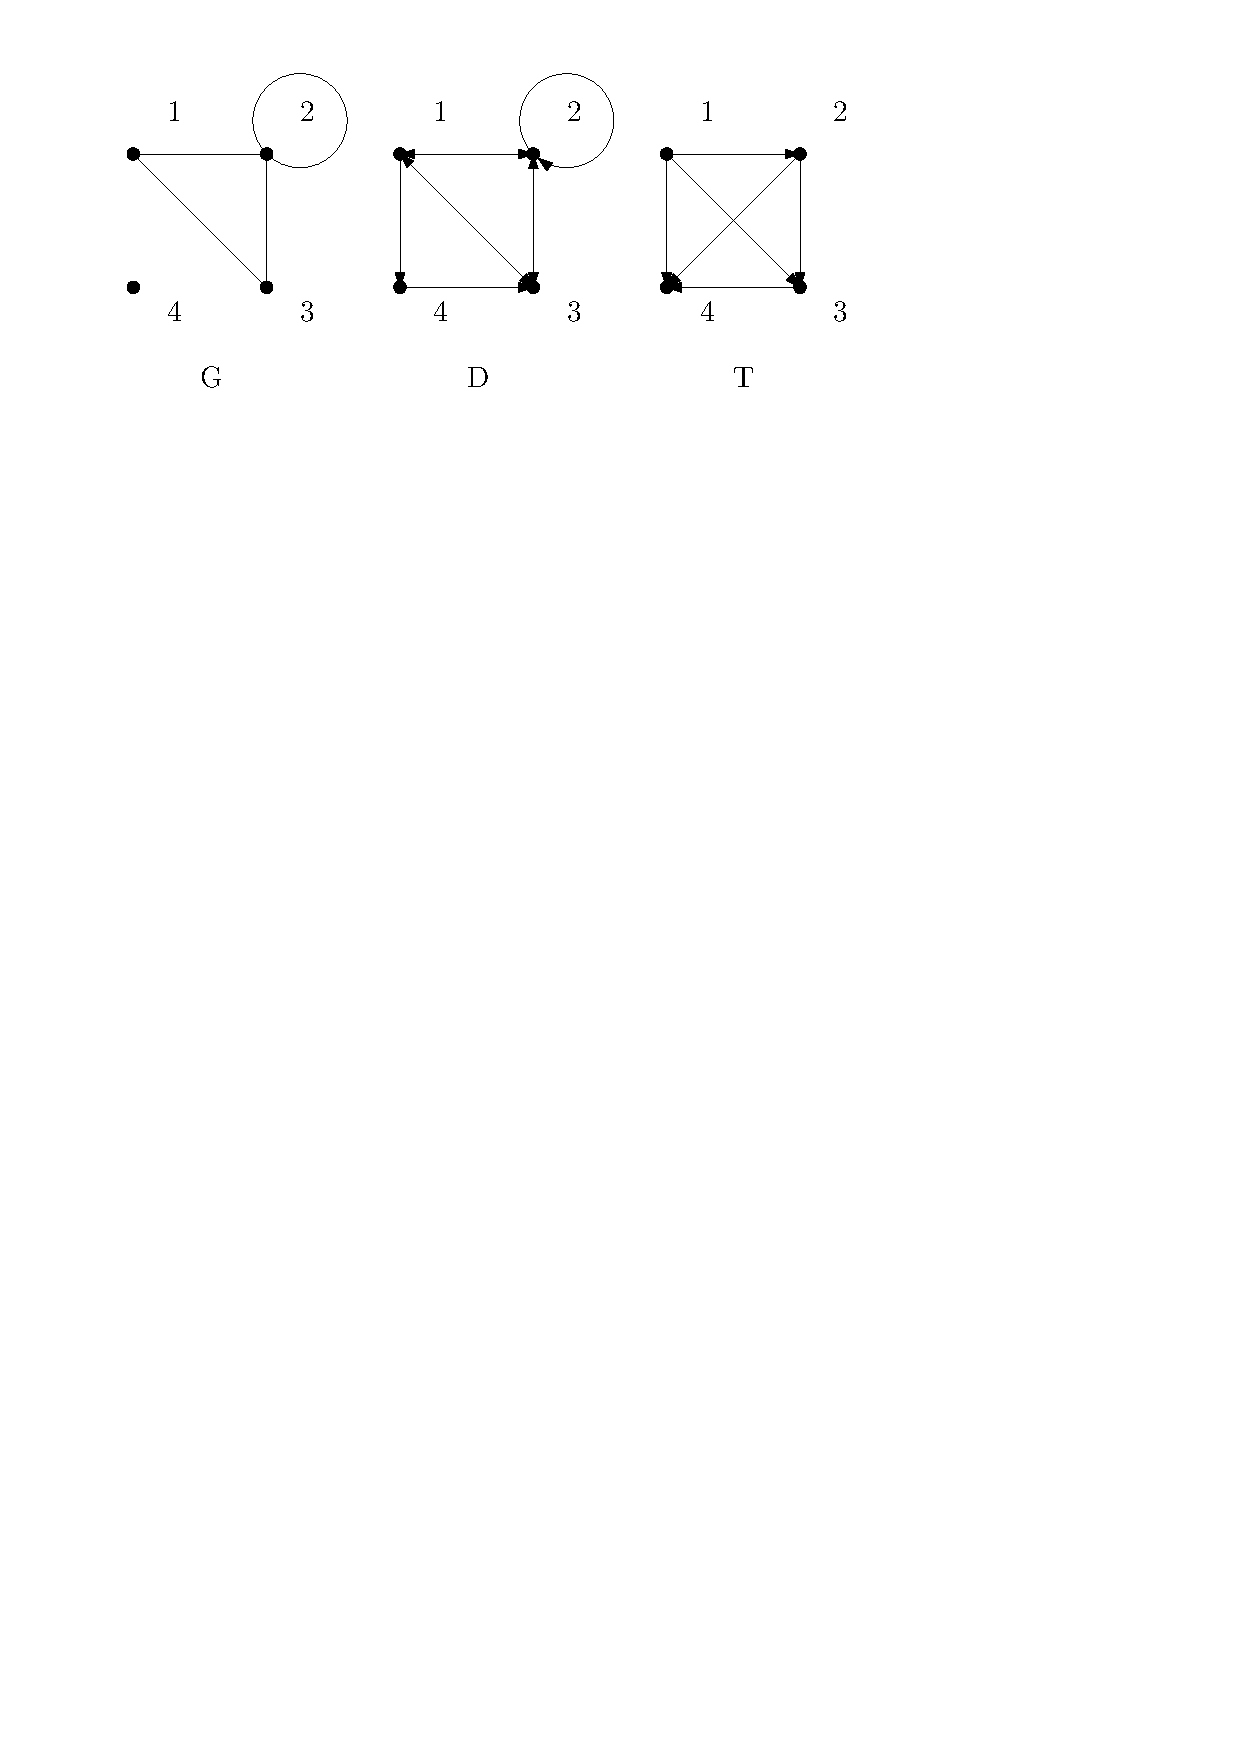
\includegraphics[scale=0.7]{app-graph}
\end{center}
\end{example}
\begin{definition}
A \textbf{path} of length $k$ in a graph or digraph is a sequence of distinct vertices $\{v_1,v_2,\ldots ,v_{k+1}\}$ such that $(v_i,v_{i+1})\in E$. A \textbf{walk} of length $k$ in a graph or digraph is a sequence of vertices $\{v_1,v_2,\ldots ,v_{k+1}\}$ such that $(v_i,v_{i+1})\in E$. A \textbf{loop} is an edge of the form $(v,v)$.
\end{definition}
\begin{example}
Let $G$ and $D$ be the graph and digraph defined above. Then we have $1,2,3$ is a path and $1,2,1,3$ is a walk and $(2,2)$ is a loop in the graph $G$. And we have $1,2,3$ is a path and $1,4,3,1$ is a walk and $(2,2)$ is a loop in the digraph $D$.
\end{example}
\begin{definition}
In a graph, \textbf{degree} of a vertex $v$, denoted by $d(v)$, is the number of edge adjacent to $v$. That is, number of elements in edge set of the form $(\cdot ,v)$. For convenience, we say that a loop contribute a vertex degree $1$. In a digraph, \textbf{out degree} of a vertex $v$, denoted by $d^+(v)$, is the number of edges of the form $(v,\cdot )$; while \textbf{in degree} of a vertex $v$, denoted by $d^-(v)$, is the number of edges of the form $(\cdot ,v)$. For convenience, we say that a loop contribute a vertex out degree $1$ and in degree $1$.
\end{definition}
\begin{example}
In the graph $G$ above, we have $d(1)=d(3)=2$, $d(2)=4$,and $d(4)=0$. In the digraph $D$ above, we have $d^+(1)=d^+(2)=3$, $d^+(3)=2$, $d^+(4)=1$ and $d^-(1)=2$, $d^-(2)=d^-(3)=3$, $d^-(4)=1$
\end{example}
\begin{definition}
For an $n\times n$ symmetric matrix $A$, we can associated a graph $\mathcal{G}(A)$ with it. The graph has vertex set $\{1,2,\ldots ,n\}$ and edge set $\{(i,j):a_{ij}\neq 0\}$. For an $n\times n$ matrix $B$, we can associated a digraph $\mathcal{G}(A)$ with it. The digraph has vertex set $\{1,2,\ldots ,n\}$ and edge set $\{(i,j):a_{ij}\neq 0\}$. And the incidence matrix of a graph is the matrix setting $a_{ij}=a_{ji}=1$ if $(i,j)$ is an edge and $a_{ij}=0$ for otherwise. And the incidence matrix of a digraph is the matrix setting $a_{ij}=1$ if $(i,j)$ is an edge and $a_{ij}=0$ for otherwise. So we have an incidence matrix with dominance relation is actually the incidence matrix of a tournament.
\end{definition}
\begin{definition}
A \textbf{clique}\footnote{This definition is different from the ``clique'' in general Graph Theory. In general, a clique means a subset of vertex of some graph such that each vertices are adjacent to each others.} is the maximal set such that each vertex connects to each others. For digraph, $v$ connect to $u$ means $(v,u),(u,v)$ are elements in the edge set.
\end{definition}
\begin{note}
By induction and some arguement, we can prove that if $A$ is incidence of a graph(digraph) then $(A^k)_{ij}$ is the number of walk from $i$ to $j$ of a graph(digraph).
\end{note}